\documentclass[../VD.tex]{subfiles}

\externaldocument{../VD}

% NEEDED REFERENCES: esferasapend (referencia pendiente a esféricas con cartas)

\begin{document}

\setcounter{chapter}{-1}

\chapter[Introducción]{Introducción a las Variedades Diferenciables}
\label{chap:intro}

Una variedad es un espacio que localmente, esto es, visto desde cerca, se
asemeja a un espacio euclídeo pero que globalmente, es decir, visto como un todo
desde ``fuera'', puede tener una estructura mucho más complicada.

El ejemplo clásico de variedad es la superficie terrestre. Nuestra percepción
local de ella es plana, pero vista desde el espacio exterior es redonda.

El tratamiento matemático de estos espacios se lleva a cabo como en la práctica
se hace al cartografiar la superficie terrestre: se eligen regiones que pueden
ser descritas por mapas euclídeos. Todos estos mapas se juntan (formando un
atlas) para describir toda la variedad teniendo en cuenta los cambios de
coordenadas al pasar de un mapa a otro.

A continuación se han seleccionado algunos ejemplos motivadores de variedades
que aparecen como espacios de configuraciones. Recordemos que en física se llama
espacio de configuraciones de un sistema mecánico $S$ al espacio $M(S)$ que
representa todas las posibles posiciones del sistema, siendo un punto de $M(S)$
la descripción completa de una posición del sistema.

\begin{description}
	
\item[Péndulo plano:] El espacio de configuraciones de este sistema es la
  circunferencia $S^{1}$: Al tomar el ángulo que forma el péndulo $P$ con una
  dirección cualquiera, los puntos en los que se puede encontrar el extremo del
  péndulo serán aquellos que tengan de radio la longitud del péndulo (que
  suponemos constante) y cualquier valor posible de ese ángulo en el intervalo
  $[0,2\pi]$. Observamos que en $0$ y en $2\pi$ el péndulo ocupa la misma
  posición, por lo que está representado por el mismo punto en el espacio de las
  configuraciones.

  \begin{figure}[ht]
    \centering
    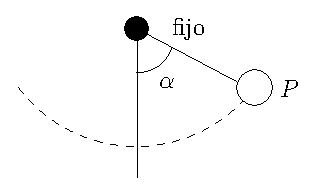
\includegraphics[scale=0.6]{intro-fig10b.eps} % NEED GRAPHICS
    \caption{}
    \label{fig10b}
  \end{figure}
  
\item[Péndulo esférico:] Para este caso el espacio será la superficie esférica
  $S^{2}$, que se obtiene de forma análoga al ejemplo anterior con otro ángulo
  más. Explícitamente, los ángulos polar (en $[0,\pi]$) y azimutal (en
  $[0,2\pi]$), que definen las coordenadas esféricas.
  % (ver \ref{esferasapend}). % TODO: Añadir referencia a atlas de la esfera.
  También quedan descritos los puntos de $S^{2}$ por medio de la latitud y la
  longitud, en los intervalos $[-\frac{\pi}{2},\frac{\pi}{2}]$ y $[0,2\pi]$,
  respectivamente. Obsérvese que para los ángulos polar $0$ y $\pi$, que
  corresponden a las latitudes $-\frac{\pi}{2}$ y $\frac{\pi}{2}$, el ángulo
  azimutal y la longitud, respectivamente, no están unívocamente definidos.

\item[Péndulo múltiple:] Dados $n$ péndulos simples (planos o esféricos)
  $P_1,\dots,P_n$, hacemos que el punto fijo del péndulo $P_{i+1}$ (llamado
  \emph{anclaje}) sea el extremo libre de $P_i$ $(1\leq i \leq n-1)$, formando
  así un nuevo mecanismo que se llama \emph{péndulo múltiple}. El espacio de
  configuraciones de este sistema será el espacio producto de los espacios de
  cada uno de los péndulos. Es decir, $S^1\times ... \times S^1$ ó $S^2 \times
  ... \times S^2$, $n$ veces.
  
  Veamos ahora una construcción explícita del espacio de configuraciones del
  péndulo doble plano. Sea $r$ la longitud del primer brazo y $s$ la longitud
  del segundo, supongamos $s<r$. Sea $O$ el anclaje del primer brazo que es el
  punto fijo del mecanismo, $P_1$ el extremo del primer brazo y anclaje del
  segundo y $P_2$ el extremo del segundo brazo.
  
  Mientras que el punto $P_1$ gira en la circunferencia de centro $O$ y radio
  $r$, el punto $P_2$ barre toda la corona circular comprendida entre las
  circunferencias concéntricas $S_-$ y $S_+$ de radios $r-s$ y $r+s$
  respectivamente; ver la Figura \ref{fig20y30}(b). Cada una de las posiciones
  de $P_2$ en el interior de la corona, sin embargo, corresponde a dos posibles
  configuraciones del péndulo doble, dependiendo si el brazo $P_1P_2$ queda a la
  derecha, o a la izquierda, del brazo $OP_1$. En contraste, cuando $P_2$ está
  sobre la circunferencia $S_+$ (o $S_-$) el brazo $P_1P_2$ debe estar
  completamente extendido apuntando hacia fuera (hacia dentro para la
  circunferencia $S_-$) y por tanto cada posición de $P_2$ en $S_+$ (y $S_-$)
  representa una única configuración. Es decir, tenemos dos copias de coronas
  pero los bordes deben ser identificados, por lo que aparece la superficie
  tórica (ver la Figura \ref{fig40y50d}(b)) que es un modelo de $S^1 \times
  S^1$. Obsérvese que si $r=s$ entonces las posiciones de $P_2$ determinan el
  círculo de centro $O$ y radio $r+s = 2r$, pero el centro de este círculo
  representa toda una circunferencia de configuraciones: aquellas
  correspondientes a cualquier posición de $P_1$ sobre la circunferencia de
  radio $r$ y el brazo $P_1P_2$ identificado con el radio de esa posición.
	
  \begin{figure}[ht]
    \centering
    \subfloat[]{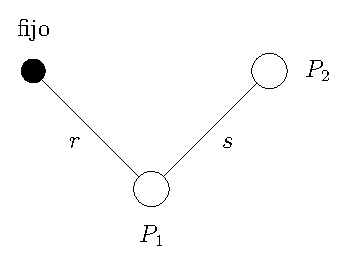
\includegraphics[scale=0.6]{intro-fig20.eps}}\qquad %% TFB % NEED GRAPHICS
    \subfloat[]{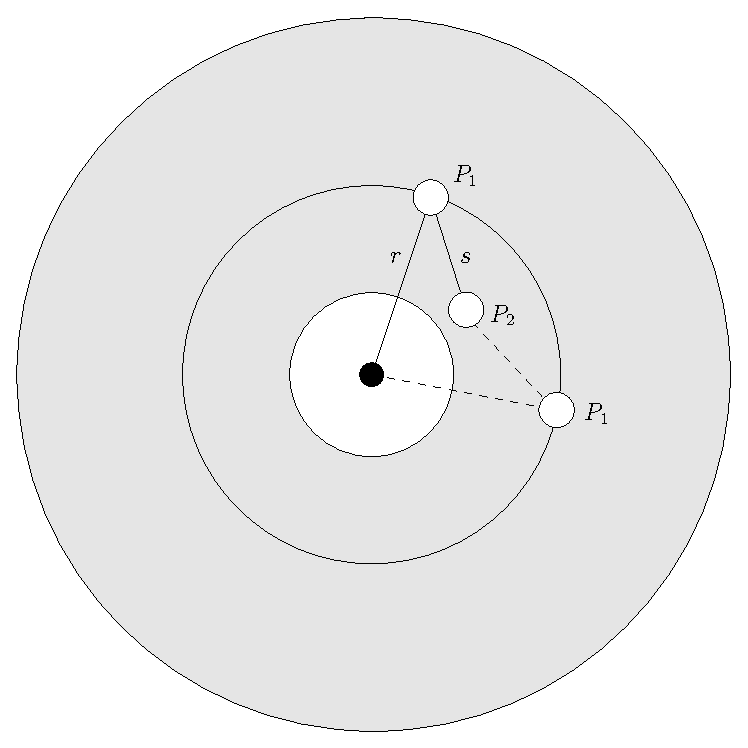
\includegraphics[scale=0.4]{intro-fig30.eps}} %% TFB % NEED GRAPHICS
    \caption{}
    \label{fig20y30}
  \end{figure}

  \begin{figure}[ht]
    \centering
    \subfloat[]{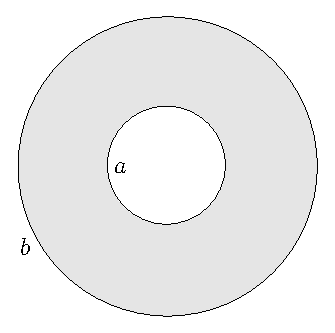
\includegraphics[scale=0.6]{intro-fig40.eps}}\qquad %% TFB % NEED GRAPHICS
    \subfloat[]{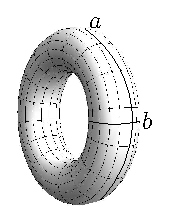
\includegraphics[scale=0.9]{intro-fig50d.eps}} %% TFB % NEED GRAPHICS
    \caption{El espacio de configuraciones del péndulo doble se obtiene al pegar las circunferencias del borde de dos copias de la corona circular, obteniéndose la superficie tórica en la derecha.}
    \label{fig40y50d}
  \end{figure}

\item[Segmento rígido:] Para definir el espacio de configuraciones de un
  segmento rígido que se mueve libremente sobre el plano necesitamos la posición
  $p\in\mathbb{R}^{2}$ de un punto cualquiera del segmento y el giro de ángulo
  $\theta\in[0,2\pi]$ que forma el segmento con una dirección elegida. Como las
  configuraciones correspondientes a los pares $(p,0)$ y $(p,2\pi)$ coinciden
  para todo $p$, el espacio de configuraciones es ahora el producto cartesiano
  $\mathbb{R}^{2}\times S^{1}$
	
\item[Triángulo rígido:] Sea $S$ el sistema mecánico formado por el triángulo
  isósceles de cateto unidad y vértices $OAB$ con un ángulo recto $\widehat{A}$
  que se mueve en torno al punto $O$ fijo; ver la Figura \ref{fig240}.

  Para determinar $M(S)$ se tiene en cuenta que el movimiento del segmento $OA$
  con $O$ fijo define una superficie esférica y una vez fijado el vector
  $\overrightarrow{OA}$ se tiene una rotación completa del vector
  $\overrightarrow{AB}$ que, por ser $\widehat{A}$ recto, forma una
  circunferencia en el plano tangente en ese punto a la superficie esférica. De
  esta forma cada posición del sistema determina unívocamente una matriz
  $3\times 3$ con primera columna $\overrightarrow{OA}$, segunda columna
  $\overrightarrow{AB}$ y tercera columna el producto vectorial de
  $\overrightarrow{OA}$ por $\overrightarrow{AB}$ en ese orden. De esta forma
  los tres vectores columna son ortonormales. Recíprocamente, dada una matriz de
  esa forma sus dos primeros vectores columna definen un punto de $M(S)$. Así
  pues $M(S)$ coincide con el conjunto de todas esas matrices, el llamado grupo
  especial ortogonal $SO(3)$, que representa a las rotaciones del espacio.

  Como cada rotación queda determinada por el par $(v,\theta)$ dado por un eje
  orientado de vector unitario $v$ y el giro de ángulo $0\leq \theta\leq 2\pi$
  (orientado respecto a $v$ por la regla del tornillo) en el plano perpendicular
  a $v$, se tiene que la rotación de eje $v$ y ángulo $\pi+\alpha$ coincide con
  la rotación de eje $-v$ y ángulo $\pi-\alpha$; en particular, los pares
  $(v,\pi)$ y $(-v,\pi)$ representan la misma rotación. Por tanto, tomando
  $0\leq \theta\leq \pi$ y viendo la rotación $(v,\theta)$ como el vector de
  módulo $\theta$ en la dirección de $v$, se puede describir $M(S)$ como la bola
  tridimensional de centro el origen y radio $\pi$ con cada punto de su borde
  identificado con su antípoda. De esta manera si $\theta$ es mayor que $\pi$ la
  rotación $(v,\theta)$ se ve en este modelo como la rotación $(-v,\theta-\pi)$,
  simétrica respecto al origen de $(v,\theta-\pi)$.

  \begin{figure}[ht]
    \centering
    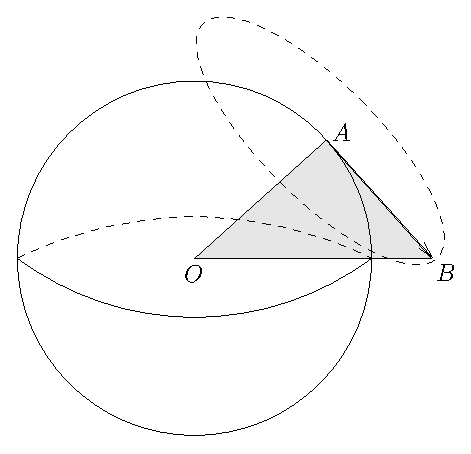
\includegraphics[scale=0.4]{intro-fig240.eps} %%TFB % NEED GRAPHICS
    \caption{}
    \label{fig240}
  \end{figure}

	Si en el ejemplo anterior el punto $O$ se deja libre en el espacio
  tridimensional entonces el nuevo espacio de configuraciones es el producto
  $\mathbb{R}^3\times SO(3)$. De hecho, éste es el espacio que nos da todas las
  posibles posiciones de cualquier sólido rígido en el espacio tridimensional.
\end{description}
  
Intuitivamente, todos los ejemplos anteriores se comportan alrededor de cada uno
de sus puntos como un espacio euclídeo, pero resulta imposible definirlos de
manera unívoca por un solo sistema de coordenadas. Así, si en $S^{2}$ se toman
como coordenadas los ángulos polar y azimutal, los polos (ángulos polares $0$ y
$2\pi$) no tienen un ángulo azimutal bien definido. Para solucionar esta
dificultad se eligen regiones que queden parametrizadas biunívocamente y se
tiene en cuenta el cambio de los parámetros al transitar de una región a otra.
Esto queda precisado en las siguientes definiciones.

\end{document}